\documentclass{article}

\usepackage{cite}
\usepackage{graphicx}
\usepackage{fancyref}
\usepackage{float}

\usepackage{listings}
\usepackage{graphicx}
\usepackage{amsmath}
\usepackage{xcolor}

\lstset{
	frame=single,
	breaklines=true,
	postbreak=\raisebox{0ex}[0ex][0ex]{\ensuremath{\color{red}\hookrightarrow\space}}
}


\title{Dynamical Systems as Gaussian Process \newline Prior Distributions}
\author{Nathan Wycoff}

\begin{document}
	
	\maketitle
	
	\section{Introduction and Background}
	
	In spatial analysis, as is often the case, different methods have been developed to solve similar problems in different applied fields. In mining and resource extraction, for instance, spatial data analysis is dominated by statistical gaussian process-like models, which developed alongside the field \cite{Krige51}. These methods are an extension of simple linear models in statistics that take spatial relationships into account.
	
	In other fields, such as biology, however, these methods are more often not used. Spatial analysis is often conducted using tools from mathematical biology, in which differential equations are derived form theory, and then integrated to make predictions about the real world (see, e.g. \cite{mathbio2}).
	 
	The world is not exactly split in this manner between math and statistics, but there is a real division between fields. The purpose of this paper is to try to merge some of the methods used in mathematical fields to Bayesian nonparametric methods with which the author is more familiar. For the unfamiliar reader, I will go over the basics of both methods we are trying to integrate in a manner which I hope reveals their possible avenues of cooperation.
	 
	 \subsection{Gaussian Processes}
	 
	 In nonparametric statistics, a Gaussian Process (GP) may be thought of as an extension of a multivariate normal distribution to uncountably many dimensions. More precisely, a GP is a distribution such that any finite sample from it has a joint normal distribution \cite{GPforML}. GP's are defined by a mean function and a covariance function (or \textit{kernel}), which define exactly what the join normal distribution that its samples' take is. 
	 
	 According to \cite{GPforML}, GP's may be thought of as "distributions over functions". The kernel function is the interesting part of the GP, as the mean may simply be removed by detrending. The kernel function can contain our \textit{a priori} beliefs about the function we are estimating. For instance, if we use a \textit{Gaussian} kernel (also referred to as a \textit{Radial Basis Function} or \textit{Squared Exponential} kernel):
	 
	 $$k(x_1,x_2) = \sigma^2 \exp{-||x_1 - x_2||_2^2 / \phi}$$
	 
	 all of our GP's realizations \textit{a posteriori} will be infinitely differentiable with probability 1 as a result of our kernel choice; we are saying that we are confident that the function we are estimating is infinitely differentiable.
	 
	 \subsection{Dynamical Systems}
	
	In applied mathematic, a Dynamical System is simply a description of a system as a function of time. This can be as simple as a closed form expression depending on time (and possibly other variables):
	
	$$y(t) = f(t,...)$$
	
	But is most often a system of differential equations with respect to time or other variables (example here is an autonomous partial differential equation):
	
	$$\frac{\partial^i y(t)}{\partial t^i} = f(\frac{\partial^i y(t)}{\partial t^i}, \frac{\partial^i y(t)}{\partial x_j^i})$$
	
	Or sometimes, in discrete math, as a system of difference equations:
	
	$$y_{t+1, j} = f(y_{t-i,j+k})$$
	
	In this paper, I will explicitly consider dynamical systems in the form of partial differential equations, but the methodology is easily extensible to any dynamical system expression.
	
	In the applied math community, there is extensive use of dynamical systems as instantiations of biological theory, as well as a way to model real data. Typically, analytical results on simplified systems are published, along with numerical results on the full systems.
	
	\subsection{Combined Learning}
	
	Work has already been done in integrating Dynamical Systems (DS) with Bayesian nonparametrics. For instance, \cite{wang2005gaussian} use GP's to average over dynamical systems, \cite{ko2007gaussian} use GP's on residuals of DS's to account for discrepancies, and \cite{solak2003derivative} use GP's to include derivative observations as data in a DS model.
	
	If kernels can be thought of as priors, can we have informative kernels? The utility of this is obvious: in general, in statistics, if one statistician has correct prior information, and the other has no prior information, the first statistician will have better results on average. In fact, the prior information need only be approximately correct (up to a certain point). 
	
	Further, it is often difficult in GP's to separate the variance from the covariance, or the signal from the noise. If a DS is accurate, it can inform our model of what the signal is because we can "observe" it without noise. Then, when we see real data, we will know that any extra variation is due to random chance. More realistically, if our DS is approximately right, we can develop an informative prior distribution on signal (represented by $\sigma^2$ in the kernel above), which will help inform our inference about the signal and noise after observing our real data.
	
	In this paper, I propose two methods to include information about a dynamical system into a GP kernel. To the best of my knowledge, the propositions that follow in this paper are novel. I have looked at some of the literature, but I have not done a full literature review, and do not claim this with absolute certainty. However, I did not come across any articles which previously implemented my propositions.
	
	\subsection{\textit{Miscellania}}
	
	In my proposal, I mentioned that I would investigate the possibility of using GP methods to numerically integrate differential equations. The integration of differential equations by GP has already been done by \cite{OHAGAN1991245}, and is referred to as \textit{Bayes-Hermite Quadrature}.
	
	\subsection{Supplementary Materials}
	
	Much code was written for this paper. As a result, not all of it is included in the appendix. However, all code may be found at the author's Github at https://github.com/NathanWycoff/SpatialFinalProject.
	
	\subsection{Outline}
	
	In Section 2, I explain the methods I will evaluate in the rest of the paper. Section 3 contains the main results of the paper, in the methods I propose are evaluated. Section 4 contains a brief data analysis component. Unfortunately, the new methods developed could not be applied to the data in Section 4, as the classification algorithm could not be made to work in a stable manner in time. This incomplete algorithm may be found in the appendix.
	
	\section{Methods}
	
	In this section I will describe the methods I will be implementing in simulations or real data analysis. In all cases, I will have a training set, on which the model estimation will occur, and a testing set, on which model evaluation will occur using Mean Square Error (MSE) for continuous valued problems, and Accuracy (1 minus mean 0-1 loss) on binary valued problems.
	
	In all the problems with which this paper is concerned, there exists subject-matter theory explaining the phenomenon which we are interested in predicting. In this paper, it will be assumed to be available in the form of differential equations, and that the differential equations' solutions are available at test and train points. These solutions may be referred to as \textit{hyperdata}.
	
	\subsection{Previously Existing Methods}
	
	\textbf{The Null Model}
	
	Simply estimate the test set with the mean or mode of the train set. Obviously, we do not expect this model to perform well. However, it is important to include, as any model performing worse than this model is completely inadmissible.
	
	\textbf{Dynamical System Prediction}
	
	Simply estimate the test set with the predictions given the dynamical system solution. This is expected to perform well when the dynamical system is approximately right, and poorly otherwise. Note that this method does not use the training set in any way.
	
	\textbf{Simple Gaussian Process}
	
	\label{simpleGauss}
	
	Simply estimate the test set using a GP fit on the training set. For this paper, I will be using a gaussian kernel with loose priors fit to the data. Particularly: 
	
	$$\sigma^2 \sim \Gamma^{-1}(0.1,0.1)$$
	
	$$\tau^2 \sim \Gamma^{-1}(0.1,0.1)$$
	
	$$ \phi \sim U(0.15, 2.5)$$
	
	Note that this method does not use the theoretical dynamical system in any way.
	
	\textbf{DS with GP on residuals}
	
	Use a GP as residuals on a linear model of the DS. Specifically:
	
	$$y(s,t) = \beta_0 + \beta_1 d(s,t) + w_{s,t}$$
	
	Where $\beta_0, \beta_1$ have uniform improper priors and $w_{s,t}$ follows a simple GP as described in the previous section.
	
	While this method takes into account both the theoretical results and the data, it does so linearly, in that one section considers the theoretical results, and the other the data, and the prediction is a compromise of the two. I believe a better method could be constructed that considers both parts in a more synergistic manner, and I will endeavor to create it in the next two sections. 
	
	\subsection{Proposition 1: Nonparametric Kernel Function}
	
	Both of my propositions involve somehow training the kernel using in part or in full the dynamical system. My first proposition is to use the covariance of the dynamical system as the covariance for the data. In practice, I integrate the differential equations at discrete points, then find the empirical covariance. I then fit a nonparametric smoother to the empirical covariance, and use this model as my kernel for a Gaussian Process model to be used on the real data. 
	
	I will follow the steps more specifically. 
	
	\begin{enumerate}
		\item Numerically integrate the dynamical system at test and train points (as well as other points if necessary).
		\item Calculate the empirical covariance. I could not find information about the empirical covariance online. Here is how I calculated it:
		
		\begin{enumerate}
			\item bins $\gets$ split($max - min$)
			\item Store pairs of points which have distances falling into each bin.
			\item Calculate sample covariance of these points.
		\end{enumerate}
		
		\item Fit a nonparametric model to the empirical covariance. To give more weight to covariances coming from new observations, duplicate observations by factor $ceil(count / min)$. For instance, if I have bins of 5, 10 and 15, and have 10 observations in the first bin, 5 in the second, and 2 in the last, we would fit a model to a kernel with 5 observations in the first bin, 3 in the second, and 1 in the last. For an example, see Figure \ref{fig1}.
		
		\item Conduct inference as usual with a GP, using the nonparametric model produced earlier as a kernel function.
		
	\end{enumerate}
	
	R code implementing the procedure may be found in the appendix.
	
	\begin{figure}[h]
		
		\caption{Example of a nonparametric kernel fit to empirical covariance, data were jittered in 2D.}
		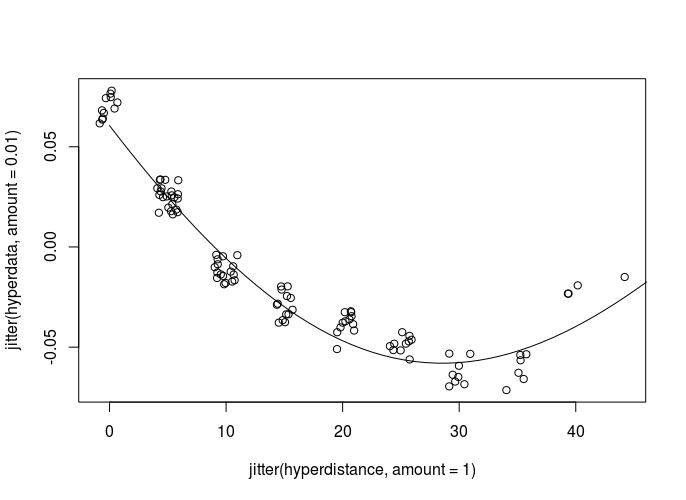
\includegraphics[scale=0.6]{FinalImage1.png}
		\label{fig1}
	\end{figure}
	
	\subsection{Proposition 2: Precondition on hyperdata}
	
	For the second method, we pick a parametric form for our kernel function as is typical in GP analysis. For this paper, I choose to use the gaussian kernel. With uninformative priors (as described in \ref{simpleGauss}), we develop a posterior on these parameters conditioned on the hyperdata. Then, we use these posteriors as priors for the real data analysis. In this way, we achieve two goals: lightly informing the prior distribution, and getting inference on $\sigma^2$ in the absence of variance. We treat the length scale parameter $\phi$ similarly. This gives us informative priors for $\sigma^2$ and $\phi$, but not for $\tau^2$. We must still use an uninformative prior for it, but it is hypothesized that estimation will be easier, as certainty about $\sigma^2$ is greater, and so will be easier to separate.
	
	I use the \textit{spBayes} package \cite{spbayes1} \cite{spbayes2} to do inference on parameters, which requires inverse gamma priors on $\sigma^2$ and $\tau^2$, and a discrete uniform prior on $\phi$. For simplicity, I moment-match the IG prior on $\sigma^2$ to its posterior \cite{llera2016estimating}, and simply use the min and max of my posterior sample on the hyperdata as the discrete uniform prior on $\phi$.
	
	
	For clarity, I include R code detailing the procedure:
	
	\begin{lstlisting}[language=R]
###
#STEP 1: Fit a GP on the PDE solution, using vague priors with no nugget effect
###
starting <- list(sigma.sq = 1, phi = 3)
tuning <- list(sigma.sq = 1, phi = 1)
priors <- list(sigma.sq.ig = c(0.1,0.1),  phi.unif = c(0.1,10)) 


precondition_fit <- spLM(DiffEQSol ~ 1, data = rbind(train,test), coords = rbind(train_coords,test_coords), starting = starting, priors = priors,
tuning = tuning, cov.model= 'gaussian', n.samples = 1000)

##Moment Match our posterior on sigma square to an IG
y <- precondition_fit$p.theta.samples[,'sigma.sq']
m <- mean(y)
v <- var(y)
alpha <- 2 + m^2 / v
beta <- m * (1 + m^2/v)

##Store our phi estimates
phi_hyper <- quantile(precondition_fit$p.theta.samples[,'phi'], c(0, 1))

###
#STEP 2: Use the new prior on sig.sq
###
starting <- list(sigma.sq = 0.1, tau.sq = 0.1, phi = 3)
tuning <- list(sigma.sq = 1, tau.sq = 1, phi = 1)
priors <- list(sigma.sq.ig = c(alpha, 1/beta), tau.sq.ig = c(0.1,0.1), phi.unif = phi_hyper)

conditioned_fit <- spLM(Observed ~ 1, data = train, coords = train_coords, starting = starting, priors = priors,
tuning = tuning, cov.model= 'gaussian', n.samples = 1000)
	\end{lstlisting}
	
	\section{Simulations}
	
	\label{sims}
	
	Since I better a computational statistician than I am a theoretical statistician, my first thought is to run simulations to evaluate my methods, and so it is what I have done. In each simulation, I integrate a "true" dynamical system, and a "used" dynamical system. The scientist then observes a noise corrupted version of the "true" system at the training points (completely randomly selected from all possible points), and uses the "used" system in models that require a dynamical system. Noise was simply iid gaussian with zero mean and standard deviation 0.1 in all cases. The scientist would then like to make inference on test locations (completely randomly selected, but may not be the same as a train location).
	
	
	\subsection{Background}
	
	In this section, a hypothetical scientist is conducting an experiment. He is standing in the middle of a field, on a day where there is no wind. He releases a gas (gas S) uniformly throughout part of the field. Gas S is not found ambiently in the field. The scientist is using a simple diffusion model to model the concentration of gas S throughout the field:
	
	$$\frac{\partial S}{\partial t} = D \Delta$$
	
	where $\Delta$ is the laplacian operator. Measurements are being made radially out from the center, and being modeled in 1 spatial dimension and 1 temporal dimension. So the laplacian operator is thus simply the second derivative w.r.t. space:
	
	$$\frac{\partial S}{\partial t} = D \frac{\partial^2 S}{\partial x^2}$$
	
	For some positive parameter D.
	
	In 3 simulations, we will explore different realities, but the scientists model will stay the same. In the first simulation, the scientist has the correct model. In the second simulation, the scientist has the wrong parameter value for D, the diffusion parameter. In the final model, the true PDE has a second component which the scientist failed to capture.
	
	Each simulation will be run with varying sample sizes many times.
	
	Obviously, the dynamical system alone will produce the most accurate estimates for the perfect model situation, and will perform worse as the truth deviates from it. The dynamical system with GP on the residuals seems to have a good balance of information and flexibility, and should perform well in most situations. The GP alone has the most flexibility, and should do better than other methods when the truth deviates substantially from the model. 
	
	The relative performance of the two new methods is of principle interest. I expect them to perform best when there is a significant deviation from the truth, but the behavior of this new system still somewhat resembles the behavior of the old system.
	
	Such a simple model is surely soluble analytically. However, in the interest of time, I used the Finite Difference Method to integrate all models in this project numerically.
	
	\subsection{Simulation 1: Perfect Model}
	
	In this simulation, the scientist's model is completely accurate, and the gas will follow its dynamics exactly:
	
	$$\frac{\partial S}{\partial t} = 10 \frac{\partial^2 S}{\partial x^2}$$
	
	 As shown in Figure \ref{fig2}, the scientist's model and the truth are the same.
	
	
	\begin{figure}[H]
		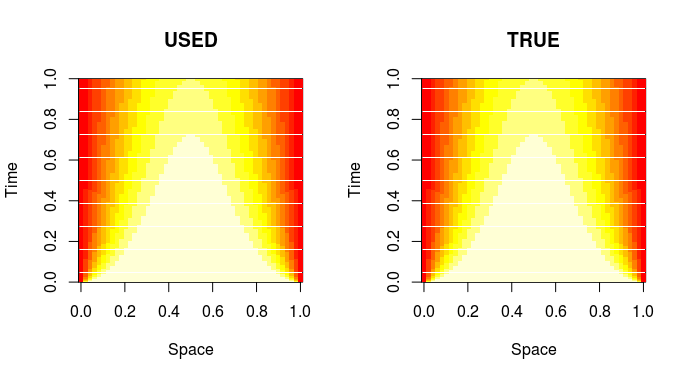
\includegraphics[scale=0.7]{FinalImage2.png}
		\caption{The PDE solutions for the used and true systems, which are the same in this simulation.}
		\label{fig2}
	\end{figure}
	
	As shown in Figure \ref{fig3}, Proposition 1 behaves terribly, having an out of sample MSE larger than the null model. Figure \ref{fig4} shows the plot with this method removed to better reveal the behavior of the other models.
	
	Figure \ref{fig4} reveals that, obviously, the dynamical system performs best, and the GP on the dynamical system also performs well. The standard GP performs about as well as the null model. Proposition 2 performs at low sample sizes similarly as the standard GP, but improves rapidly as sample size increases, never quite reaching the ability of the dynamical system.
	
	\begin{figure}[H]
		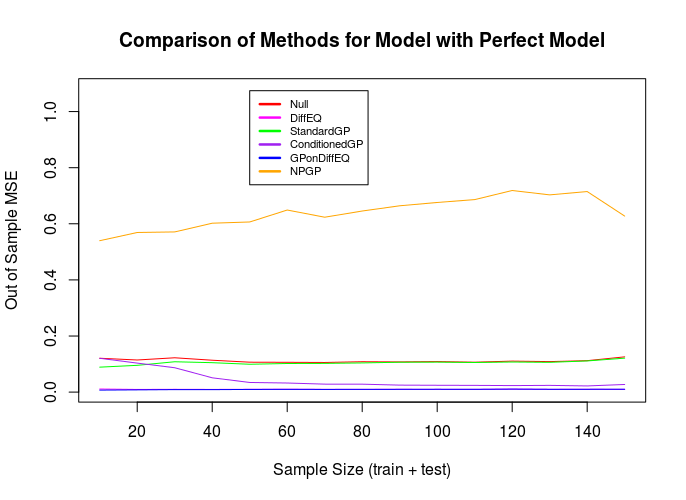
\includegraphics[scale=0.7]{PrezImage4.png}
		\caption{The performance of all models over varying sample sizes. Null is the null model, DiffEQ is the dynamical system, ConditionedGP is Proposition 2, GPonDiffEQ is the GP on the residuals of the dynamical system, and NPGP is Proposition 1.}
		\label{fig3}
	\end{figure}
	
	\begin{figure}[H]
		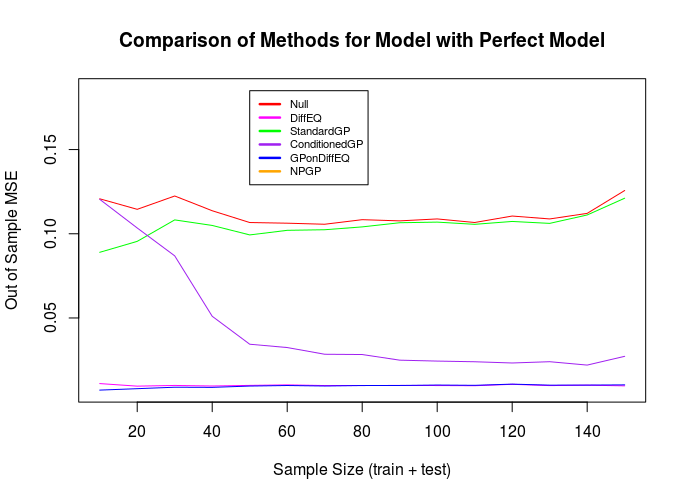
\includegraphics[scale=0.7]{PrezImage5.png}
		\caption{The performance of all models except NPGP over varying sample sizes.}
		\label{fig4}
	\end{figure}
	
	
	\subsection{Simulation 2: Parameter Error}
	
	In this simulation, the scientist's model is close to the truth, but he has one of the parameters off.
	
	True Model:
	
	$$\frac{\partial S}{\partial t} = 10 \frac{\partial^2 S}{\partial x^2}$$
	
	Scientist's model:
	
	$$\frac{\partial S}{\partial t} = 30 \frac{\partial^2 S}{\partial x^2}$$
	
	
	\begin{figure}[H]
		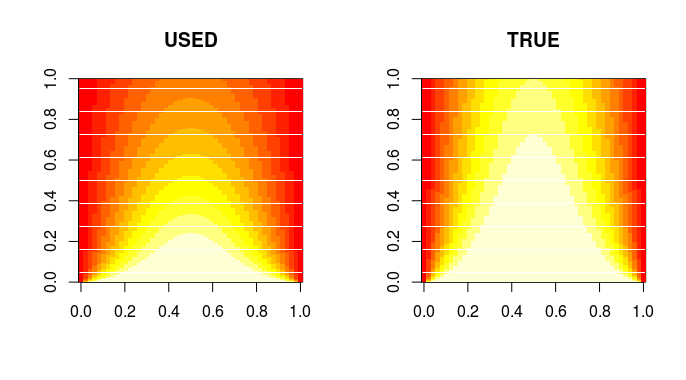
\includegraphics[scale=0.7]{FinalImage3.png}
		\caption{The PDE solutions for the used and true systems. The scientist believes the diffusion is much quicker than it is.}
		\label{fig7}
	\end{figure}
	
	Proposition 1 again fairs terribly, and is left out of Figure \ref{fig8}. The standard GP is again about as bad as the null model. The pure dynamical system predictions this time fall predictably short. As last time, Proposition 2 at first behaves terribly, but for larger sample sizes, rivals the DS with GP residuals, which is consistently the best.
	
	\begin{figure}[H]
		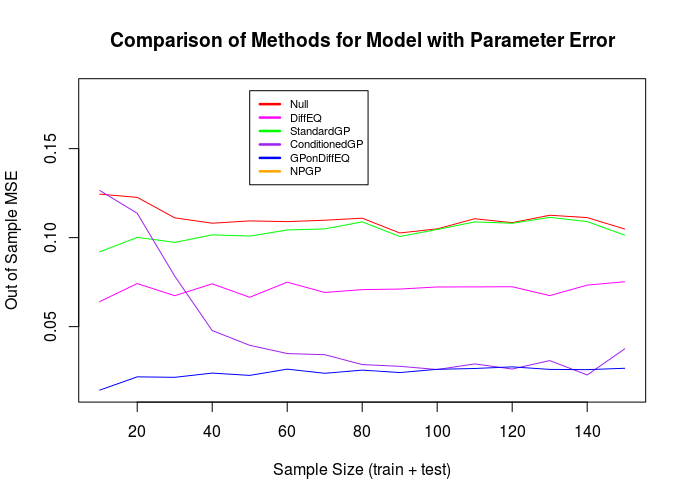
\includegraphics[scale=0.7]{PrezImage3.png}
		\caption{The performance of all models over varying sample sizes. Null is the null model, DiffEQ is the dynamical system, ConditionedGP is Proposition 2, GPonDiffEQ is the GP on the residuals of the dynamical system, and NPGP is Proposition 1.}
		\label{fig8}
	\end{figure}
	
	\subsection{Simulation 3: Structural Error}
	
	In this simulation, the scientist's model has a structural deviation from the truth. For instance, perhaps there is some naturally occurring gas R which bonds with gas S at a slow rate to turn into some third gas which does not interact with these two. As gas R is naturally occurring, we model it as having a constant spread over the space of interest, and as having constant boundary conditions.
	
	Scientist's Model:
	
	$$\frac{\partial S}{\partial t} = 10 \frac{\partial^2 S}{\partial x^2}$$
	
	\vspace{1em}
	
	Truth:
	
	$$\frac{\partial S}{\partial t} = 10 \frac{\partial^2 S}{\partial x^2} - 0.05 S R$$
	
	$$\frac{\partial R}{\partial t} = 10 \frac{\partial^2 R}{\partial x^2} - 0.05 S R$$
	
	Though the truth is a system of equations, we are only explicitly interested in the behavior of S. 
	
	
	\begin{figure}[H]
		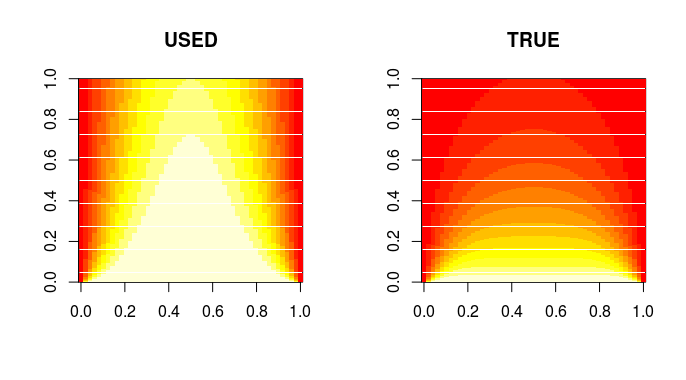
\includegraphics[scale=0.7]{FinalImage4.png}
		\caption{The PDE solutions for the used and true systems. The scientist's model is substantially different from reality.}
		\label{fig9}
	\end{figure}
	
	Proposition 1 performs much better comparatively in this model, though this is only because the dynamical system does so poorly. GP on DS residuals and the standard GP behave as before. Excitingly, Proposition 2 performs best out of all models for several sample sizes.
	
	\begin{figure}[H]
		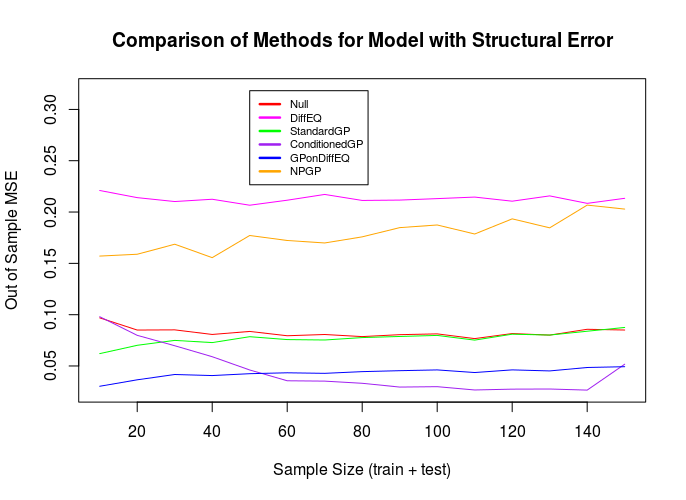
\includegraphics[scale=0.7]{PrezImage1.png}
		\caption{The performance of all models over varying sample sizes. Null is the null model, DiffEQ is the dynamical system, ConditionedGP is Proposition 2, GPonDiffEQ is the GP on the residuals of the dynamical system, and NPGP is Proposition 1.}
		\label{fig10}
	\end{figure}
	
	\subsection{Discussion}
	
	Proposition 1 fairs very poorly in all simulations. I am not sure exactly why this is. Perhaps the issue is that it is trained on data that do not have any variance, and has no "nugget effect" to explain excess variance on the real data. Perhaps it simply overfits to hyperdata, or perhaps it is not flexible enough for to adjust to the real data like the other models do. In any event, it performs extremely poorly, and I would not advocate its serious use in any context.
	
	Proposition 2 is a much more interesting story. In situations where we know the model perfectly, it is obviously best to simply use the true model. However, this situation rarely arises in reality. The more interesting scenarios are thus simulations 2 and 3, where we have the correct structure, but incorrect parameters, and simulation 3, where we have incorrect structure, perhaps the most realistic scenario; surely we rarely have a perfect understanding of a system's dynamics.
	
	In simulation 2, Proposition 2 quickly catches up with the GP on the dynamical system's residuals. In simulation 3, Proposition 3 actually beats the the existing methods for sample sizes greater than 50, which is extraordinarily exciting. The gap only expands as the sample size increases, before becoming equal at 150. I believe the equality at 150 is the result of a simulation error. As the sample size increases, spBayes has a higher change of throwing errors during the phase where the kernel is fit to the hyperdata. I believe it has issues fitting models with no nugget if some of the training data are too close together. However, further study is necessary to confirm this suspicion. 
	
	In Bayesian statistics in general, correct prior information is most advantageous at small sample sizes. As the methods proposed here are meant to encode dynamical system information as prior knowledge, a natural question to ask is thus "Why does the sample size need to increase before Proposition 2 is efficient?". Propositions 1 and 2 use dynamical system solution information at all train and test points. It is probable that a large number of dynamical solution solutions are required in order for its dynamics to be learnt. Obviously, dynamical system solutions may be obtained at many more places than at training points. Perhaps a modified Proposition 2, where the dynamical system solution is used not only at training and testing points, but also near them, would work at lower sample sizes.
	
	Though these simulations were in $R^2$, they only had 1 spatial dimension. I believe that this is easily extensible to the 2D case which is canonical in spatial analysis.
	
	\section{Real Data Analysis}
	
	In this section, I will do a brief analysis of some real world bivariate binary spatiotemporal data. Unfortunately, I did not develop stable implementations of my Propositions for classification in $R^3$ in time for this project, which is where my data in this section lie. As such, Propositions 1 and 2 will not be referenced in this section, against my original intentions. 
	
	\subsection{Background}
	
	In much of Britain, the native Red Squirrel has been pushed out of its habitat by the American Grey Squirrel, an alien species introduced there \cite{gurnellsquirrel}. The grey squirrel is used to competition from other squirrel species in the US, and so is more fit in the Darwinian sense than is the native red squirrel which until recently had no competitor species. Grey squirrels are also present in mainland Europe. Of great interest to ecologists is to be able to predict the spread of the grey squirrel and the disappearance of the red squirrel. \cite{reynolds1985details} has data on the spread of squirrels in eastern Britain which, in the absence of computer records, I have painstakingly translated into an R array. As my "used" dynamical system, I use the Lotka-Volterra \cite{goellotka} diffusion model used in \cite{okubo1989spatial}:
	
	$$\frac{\partial G}{\partial t} = D_1 \Delta G + a_1 G (1 - b_1 G - c_1 R)$$ 
	
	$$\frac{\partial R}{\partial t} = D_2 \Delta R + a_2 R (1 - b_2 G - c_2 G)$$
	
	Here, $D_1,D_2$ denote the diffusion rates, $a_1,a_2$ the reproduction rates, $b_1,b_2$ the inverse carrying capacities, and $c_1,c_2$ the competition coefficients. \cite{okubo1989spatial} suggest values for all of these rates except for $c_1, c_2$, which they remove through nondimensionalization. However, playing with different values, the system does not seem to vary significantly as $c_1,c_2$ change. I set them equal in my case. The authors of \cite{okubo1989spatial} use zero flux boundary conditions. However, these don't make sense to me. I believe constant boundary conditions make the most sense. In \cite{parker2008gray}, red squirrel density in areas occupied only be red squirrels was estimated to be 0.39/ha based on Capture Mark Recapture methods. As such, I set the initial and boundary conditions of the red squirrel to be 0.39 everywhere. Initial conditions for the grey squirrel was a point mass of 1 in the middle, and values of zero everywhere else and at the boundaries. This system was again solved using the Finite Difference Method.
	
	Figure \ref{fig11} shows the data from \cite{reynolds1985details}. Note that the data are coded in grid squares, so a Markov Random Field is probably a better model than a Gaussian Process. However, since it is more obvious to me how to use Dynamical System information with a GP than with a MRF, I will use a GP, treating the data as a grid of continuous observations.
	
	\begin{figure}[H]
		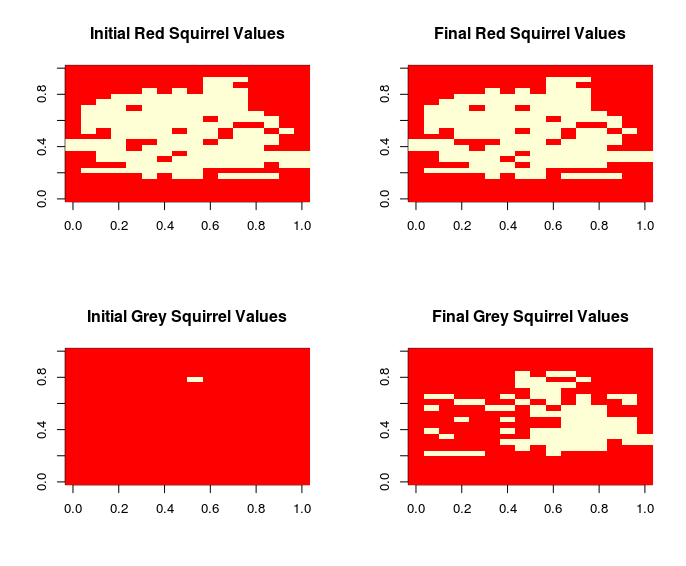
\includegraphics[scale=0.6]{FinalImage5.png}
		\caption{The initial and final spatial locations of squirrels.}
		\label{fig11}
	\end{figure}
	
	\subsection{Methods}
	
	In this section, we compare two methods.
	
	The solution to our dynamical system is continuous, but we have a dichotomous response. As such, we simply use logistic regression as representative of our "only DS" route. We use a GP for classification as representative of the "only GP" model. It is not as obvious to me how to build a GP on the "residuals" of the DS model, as residuals do not exist in a binary response model as they do in a continuous response model.
	
	To evaluate the predictive ability of the model, we simply do 1 step forward prediction over the entire grid.
	
	\subsection{Results}
	
	As is shown in the table below, the GP beat the DS at every turn. As I hoped to show in Section \ref{sims}, however, there may be much to be gain in combining the two methods.
	
	This table measures predictive 1 step ahead accuracy for each model:
	
	\begin{center}
		\begin{tabular}{ c c c }
			Model & MSE Grey & MSE Red \\ 
			DS & 0.57 & 0.83 \\  
			GP & 0.86 & 0.86
		\end{tabular}
	\end{center}
	
	
	
	\bibliography{final}{}
	\bibliographystyle{plain}
	
	\section{Appendices: R Scripts}
	
	\textbf{Script 1}
	
	This script contains a working version of Proposition 1 for regression.
	
	\begin{lstlisting}[language=R]
#Do GP regression (Point estimates only), using a kernel function
# nonparametrically fit to solutions of a dynamical system
#
# X -- Locations of training data
# y -- Response at locations
# XX -- Locations to predict at
# solx -- solution of dynamical system at training points
# solxx -- solution of dynamical system at testing points
nathans_gp_reg <- function(y, X, XX, solx, solxx) {
#####
## Do hyper GP
#####

XXX <- rbind(X,XX)

##Get Covariance
D <- dist(XXX)#Create a distance matrix
bins <- hist(D, plot = FALSE)$breaks#create bins

#Go over it all and get the covariances.
n <- dim(XXX)[1]
covs <- c()
lens <- c()
hyperdistance <- c()
for (bi in 1:(length(bins)-1)) {
y1 <- c()
y2 <- c()
b <- bins[bi+1]
b1 <- bins[bi]
for (j in 1:n) {
for (i in 1:j) {
if (i == j) {
next
}
ind <- n*(i-1) - i *(i-1)/2 + j - i
if (D[ind] < b && D[ind] >= b1) {
y1 <- c(y1, c(solx, solxx)[i])
y2 <- c(y2, c(solx, solxx)[j])
}
}
}
if (length(y1) > 1) {
covs <- c(covs, cov(y1,y2))
lens <- c(lens, length(y1))
hyperdistance <- c(hyperdistance, b1)
}
}

#Use weights to get multiple points for bin in the histo
weights <- floor(lens / min(lens))#Weigh cov estimates approximately by their number of constituents.
hyperdata <- rep(covs,weights)
hyperdistance <- rep(hyperdistance,weights)

##Get rid of places with only one datum
#hyperdata <- hyperdata[which(rep(weights > 1, weights))]
#hyperdistance <- hyperdistance[which(rep(weights > 1, weights))]

#Fit GP to these covars
length_scale <- (bins[2] - bins[1])*1000#Make the length scale 1 bin
gpi <- newGP(matrix(hyperdistance), hyperdata, d=length_scale, g=0.1, dK=FALSE)
ga <- garg(list(mle=TRUE, min =0.01, max=15, start = 5), hyperdata)  #Make max bigger?
mle<-mleGP(gpi, param="g", tmin=ga$min, tmax=ga$max, ab=ga$ab)
grid <- matrix(seq(min(hyperdistance), max(hyperdistance)*5, length.out = 250))
p <- predGP(gpi, grid, lite=TRUE)$mean

#Visualize nonparam kernel
plot(jitter(hyperdistance,amount=1), jitter(hyperdata, amount = 0.01))
points(grid, p, type = 'l')

#Store the predicted values and spit out each step.
np_k <- function(x1,x2) {
#print("hehehoho")
#print(x1)
h <- norm(x1 - x2, '2')
return(p[min(which(grid > h))])
}

##Create Covariance Matrix
n <- length(y)
K <- matrix(rep(0, n*n), nrow = n)
for (i in 1:n) {
for (j in 1:n) {
K[i,j] <- np_k(X[i,], X[j,])
}
}

##Do prediction
sigma2 <- 10

#Some precacluations
L <- chol(K + diag(sigma2, n))
alpha <- solve(t(L), solve(L, y))

#Iterate over each data point and spit out our predictions
f <- c()
for (i in 1:dim(XX)[1]) {
x_new <- XX[i,]
k_new <- sapply(1:dim(X)[1], function(j) np_k(x_new, X[j,]))
f <- c(f, t(k_new) %*% alpha)
}

return(f)
}
	\end{lstlisting}
	
	\textbf{Script 2}
	
	This script contains a non-working version of Proposition 1 for Classification using the Laplace Approximation.
	
	\begin{lstlisting}[language=R]
#Do GP Classification (Point estimates only), using a kernel function
# nonparametrically fit to solutions of a dynamical system
#
# X -- Locations of training data
# y -- Response at locations
# XX -- Locations to predict at
# solx -- solution of dynamical system at training points
# solxx -- solution of dynamical system at testing points
nathans_gp_class <- function(y, X, XX, solx, solxx) {
#####
## Do hyper GP
#####

XXX <- rbind(X,XX)

##Get Covariance
D <- dist(XXX)#Create a distance matrix
bins <- hist(D, plot = FALSE)$breaks#create bins

#Go over it all and get the covariances.
n <- dim(XXX)[1]
covs <- c()
lens <- c()
for (bi in 1:(length(bins)-1)) {
y1 <- c()
y2 <- c()
b <- bins[bi+1]
b1 <- bins[bi]
for (j in 1:n) {
for (i in 1:j) {
if (i == j) {
next
}
ind <- n*(i-1) - i *(i-1)/2 + j - i
if (D[ind] < b && D[ind] >= b1) {
y1 <- c(y1, c(solx, solxx)[i])
y2 <- c(y2, c(solx, solxx)[j])
}
}
}
covs <- c(covs, cov(y1,y2))
lens <- c(lens, length(y1))
}

#Use weights to get multiple points for bin in the histo
weights <- floor(lens / min(lens))#Weigh cov estimates approximately by their number of constituents.
hyperdata <- rep(covs,weights)
hyperdistance <- rep(bins[2:length(bins)],weights)

#Fit GP to these covars
length_scale <- (bins[2] - bins[1])*1000#Make the length scale 1 bin
gpi <- newGP(matrix(hyperdistance), hyperdata, d=length_scale, g=0.1, dK=FALSE)
ga <- garg(list(mle=TRUE, min =0.01, max=15, start = 5), hyperdata)  #Make max bigger?
mle<-mleGP(gpi, param="g", tmin=ga$min, tmax=ga$max, ab=ga$ab)
grid <- matrix(seq(min(hyperdistance), max(hyperdistance)))
p <- predGP(gpi, grid, lite=TRUE)$mean

#Visualize nonparam kernel
plot(jitter(hyperdistance,amount=1), jitter(hyperdata, amount = 0.1))
points(grid, p, type = 'l')

#Store the predicted values and spit out each step.
np_k <- function(x1,x2) {
#print("hehehoho")
#print(x1)
h <- norm(x1 - x2, '2')
return(p[min(which(grid > h))])
}

#Our covar mat
K <- matrix(rep(0, n*n), nrow = n)
for (i in 1:n) {
for (j in 1:n) {
K[i,j] <- np_k(X[i], X[j])
}
}


##Begin Laplace Approx Algorithm from Rasmussen and Williams pg 46
get_mode <- function(K, y) {
n <- length(y)
#Initializations
f <- rnorm(n,0,0.1)

#Newton iteration
tol <- 0.1
while (TRUE) {

##Update our stuff
W <- diag(pnorm(train$y * as.numeric(f)) * (1-pnorm(y * as.numeric(f))))
L <- chol(diag(n) + sqrt(W) %*% K %*% sqrt(W))
b <- W %*% f + (y+1)/2 - pnorm(y*f)
a <- b - sqrt(W) %*% solve(t(L), solve(L, sqrt(W) %*% K %*% b))
f_new <- K %*% a

##Check for convergence
if (norm(f_new - f, 'I') < tol) {
break
}
f <- f_new
}
return(f)
}

##Prediction using laplace approx
laplace_predict <- function(f, X, XX, y) {
#k_new <- t(sapply(test$X, function(x_new) sapply(train$X, function(x) k(x_new, x))))
f_new <- c()
for (x_new in XX) {
W <- diag(pnorm(y * as.numeric(f)) * (1-pnorm(y * as.numeric(f))))
L <- chol(diag(n) + sqrt(W) %*% K %*% sqrt(W))
k_new <- sapply(X, function(x) k(x_new, x))
###############################################
jacob_diag <- (train$y+1)/2 - pnorm(train$y*f)
f_new <- c(f_new, t(k_new)  %*% jacob_diag)
###############################################
}
return(f_new)
}

f <- get_mode(K, y)

f_pred <- laplace_predict(f, X, XX, y)

return(f_pred)
}
	\end{lstlisting}
	
\end{document}